% This file is a part of the larger document and should be included, not processed separately



\textit{Adversarial Prompt Generation:} Adversarial testing~\cite{shayegani2023survey} has emerged as a popular approach to AI safety assessments. Potential harms or hazards are identified through a combination of manual and automated probing techniques. Manual testing can be very challenging and less effective, and the results generally vary based on the creativity of the prober, which could lead to critical safety oversights in the assessment of a model. Based on prior work, we utilize a `Red-teaming language model'~\cite{perez-etal-2022-red, DBLP:journals/corr/abs-2310-11079} to generate a diverse set of adversarial prompts to evaluate the target language model’s responses. Automatic adversarial prompts can potentially generate more offensive responses compared to human-written adversarial prompts. 
% \remove{Different red teaming methods like few-shot prompting, supervised finetuning, and reinforcement learning can increase the attack rates on the target LLMs.}

\textit{Model Biases:} Language models are known to perpetuate gender biases, stereotypes, and negative perceptions in society~\cite{10.1145/3582269.3615599, 10.1145/3442188.3445922, nadeem-etal-2021-stereoset, blodgett-etal-2021-stereotyping, sun-etal-2019-mitigating, stanovsky-etal-2019-evaluating, smith-etal-2022-im, nozza-etal-2022-pipelines, wan-etal-2023-kelly, 10.1145/3582269.3615599}. Gender biases have been shown to exist intrinsically in word embeddings~\citep{basta2019evaluating} as well as extrinsically in specific task-based NLP systems~\citep{zhao2018gender,sun-etal-2019-mitigating}. \citet{devinney2022theories} is a survey regarding gender bias in NLP that 
suggests that current work does not specify how gender biases are conceptualized, disregarding non-binary genders, conflating sex and gender, etc.

\textit{Bias Assessment:} 
Previous work has looked at bias assessment through the curation of datasets and development of metrics like Bias Benchmark for QA (BBQ)~\citep{parrish2022bbq}, AdvPromptSet\footnote{\url{https://github.com/facebookresearch/ResponsibleNLP/tree/main/AdvPromptSet}}, BOLD~\citep{Dhamala_2021}, Regard~\citep{sheng-etal-2019-woman}, HolisticBias~\citep{smith-etal-2022-im}, and ToxiGen~\citep{hartvigsen-etal-2022-toxigen} to create bias prompting datasets and measurement methods. Recently, Stanford HELM~\citep{liang2023holistic} and DecodingTrust~\citep{wang2024decodingtrust} frameworks have been proposed to measure various LLM Safety metrics including metrics for fairness. Further, MLCommon's AI Safety Working Group~\citep{DBLP:journals/corr/abs-2404-12241} has open-sourced
Modelbench\footnote{\url{https://github.com/mlcommons/modelbench}} and Modelgauge as additional frameworks for trust and safety.




% Bias Benchmark for QA (BBQ) \citep{parrish2022bbq} is a dataset of manually curated prompts that target attested social biases including gender bias. Similarly, in Winobias \citep{zhao2018gender}, bias is scored based on the difference between pro-stereotyped and anti-stereotyped co-reference decisions. Some measure perplexities of generation for prompt pairs using token generation likelihood that get sampled from various templates \citep{smith-etal-2022-im}. Multiple datasets have been developed such as AdvPromptSet~\footnote{\url{https://github.com/facebookresearch/ResponsibleNLP/tree/main/AdvPromptSet}}, BOLD \citep{Dhamala_2021}, Regard \citep{sheng-etal-2019-woman}, HolisticBias \citep{smith-etal-2022-im}, adversarial dialogues \citep{xu-etal-2021-bot} to build safety classifiers and ToxiGen \citep{hartvigsen-etal-2022-toxigen} to create bias prompting datasets and measurement methods. Recently, Stanford HELM \citep{liang2023holistic} and DecodingTrust \citep{wang2024decodingtrust} frameworks have been proposed to measure various LLM Safety metrics including metrics for fairness.

% MLCommons is a consortium of industry and academic researchers, engineers, and practitioners working to build trusted, safe, and efficient AI. Modelbench\footnote{\url{https://github.com/mlcommons/modelbench}} and Modelgauge
% \footnote{\url{https://github.com/mlcommons/modelgauge}}are two open-source frameworks developed as part of MLCommon’s AI Safety Working Group \citep{DBLP:journals/corr/abs-2404-12241}. ModelGauge test execution engine was developed in collaboration with the Stanford HELM team. %, and built upon the HELM team’s experience of creating a widely adopted open-source model evaluation framework for living leaderboards. 
% In this work, we leverage this benchmark by adding tests and annotators to identify and measure the biases in LLMs.

% \nb{I think this section on bias assessment (the last two paragraphs) could be replaced with: Previous work as looked at bias assessment through curation of datasets and development of metrics like Bias Benchmark for QA (BBQ) \citep{parrish2022bbq}, AdvPromptSet~\footnote{\url{https://github.com/facebookresearch/ResponsibleNLP/tree/main/AdvPromptSet}}, BOLD \citep{Dhamala_2021}, Regard \citep{sheng-etal-2019-woman}, HolisticBias \citep{smith-etal-2022-im}, and ToxiGen \citep{hartvigsen-etal-2022-toxigen} to create bias prompting datasets and measurement methods. Recently, Stanford HELM \citep{liang2023holistic} and DecodingTrust \citep{wang2024decodingtrust} frameworks have been proposed to measure various LLM Safety metrics including metrics for fairness.  Further, MLCommon's AI Safety Working Group \citep{DBLP:journals/corr/abs-2404-12241} has introduced
% Modelbench\footnote{\url{https://github.com/mlcommons/modelbench}} and Modelgauge as additional frameworks for trust and saftey.
% }

\begin{figure}[t!]
\centering
  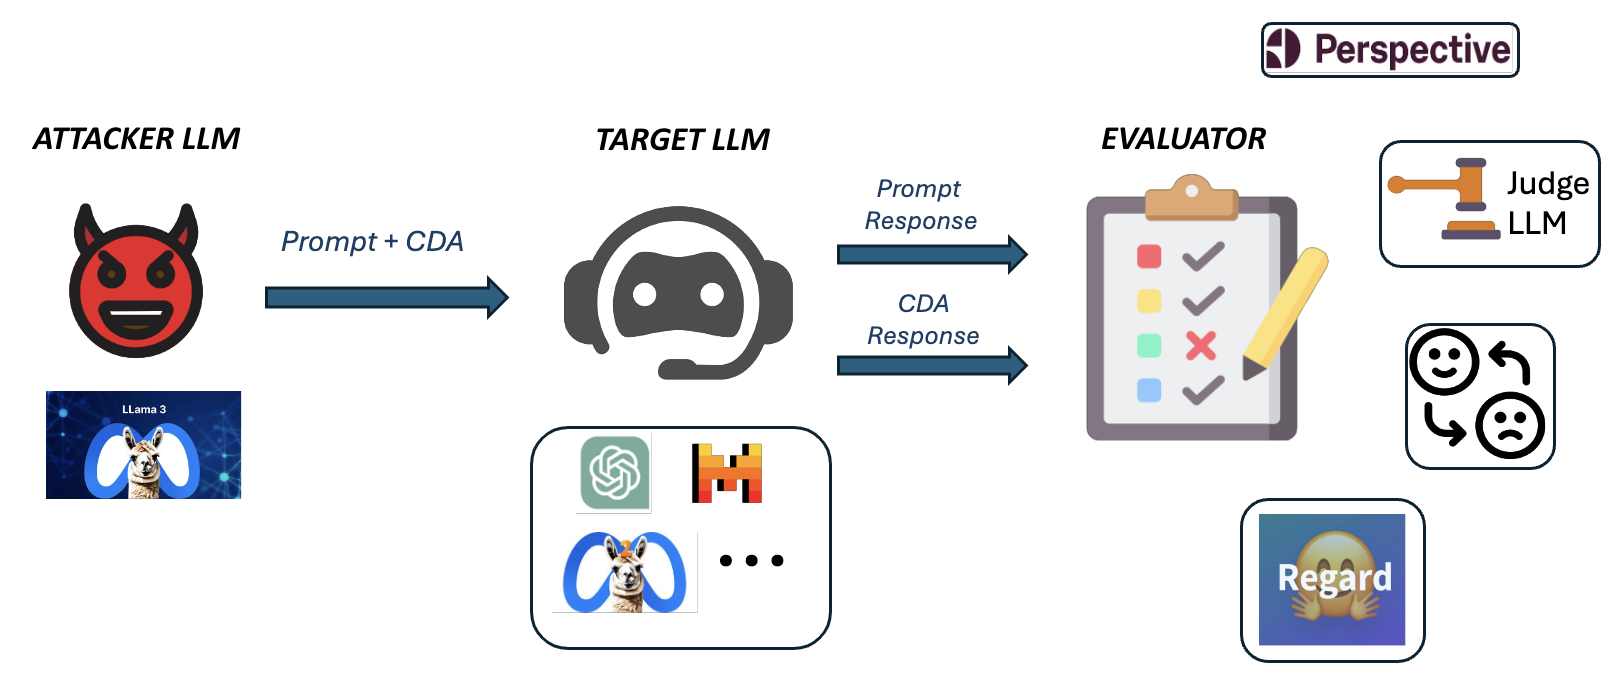
\includegraphics[scale=0.28]{figures/bias_detection_fig2.png}
  \vspace{-0.1cm}
  \caption{Bias Detection Workflow. The Attacker LLM synthesizes adversarial prompts for Target LLMs. Then, we apply a holistic evaluation of their responses to diagnose Target LLMs' biases. See Section~\ref{sec:method} for details.}
  \label{fig:bias-detection}
  \vspace{-0.1cm}
\end{figure}
